% https://tex.stackexchange.com/a/767245
\documentclass[tikz,border=3.14pt]{standalone}
\usepackage{newtx}
\usetikzlibrary{arrows.meta,decorations.pathreplacing}

\definecolor{ink}{RGB}{43,42,39}
\definecolor{axisink}{RGB}{67,65,60}
\definecolor{hiddenink}{RGB}{157,161,148}
\definecolor{domainfill}{RGB}{254,219,180}
\definecolor{domainrim}{RGB}{245,169,60}
\definecolor{surfaceleft}{RGB}{158,216,241}
\definecolor{surfaceright}{RGB}{43,174,215}
\definecolor{surfacerim}{RGB}{48,186,223}

% Surface outline: 21 fitted cubic Bezier segments.
\def\surfaceoutline{%
    (383.69,108.03)
    .. controls (322.77,110.28) and (265.19,125.91) .. (212.37,149.82)
    .. controls (197.30,156.65) and (182.61,164.14) .. (169.63,175.11)
    .. controls (155.75,186.83) and (143.82,202.52) .. (133.83,217.88)
    .. controls (125.05,231.36) and (117.76,244.59) .. (115.59,260.76)
    .. controls (114.61,268.03) and (114.66,275.88) .. (117.65,281.76)
    .. controls (120.85,288.07) and (127.42,292.10) .. (134.36,293.51)
    .. controls (148.28,296.35) and (163.66,288.62) .. (177.83,281.61)
    .. controls (192.96,274.11) and (206.72,267.44) .. (220.64,260.01)
    .. controls (247.56,245.64) and (275.13,228.46) .. (305.68,221.34)
    .. controls (319.60,218.10) and (334.14,216.95) .. (348.37,218.41)
    .. controls (362.81,219.89) and (376.95,224.07) .. (390.45,229.43)
    .. controls (420.97,241.55) and (448.25,259.74) .. (475.25,279.04)
    .. controls (528.23,316.91) and (580.16,359.03) .. (646.42,364.58)
    .. controls (661.01,365.80) and (676.29,365.25) .. (689.82,360.89)
    .. controls (705.82,355.74) and (719.36,345.27) .. (728.63,330.99)
    .. controls (736.90,318.26) and (741.78,302.49) .. (740.71,287.56)
    .. controls (739.64,272.42) and (732.47,258.14) .. (723.43,245.51)
    .. controls (702.52,216.30) and (671.64,195.93) .. (640.45,179.27)
    .. controls (612.41,164.30) and (584.13,152.32) .. (555.33,141.08)
    .. controls (527.78,130.32) and (499.76,120.24) .. (469.61,114.32)
    .. controls (441.92,108.89) and (412.43,106.97) .. (383.69,108.03)
    -- cycle
}

% Domain outline: 22 fitted cubic segments shared by fill and stroke.
\def\domainoutline{%
    (235.54,436.25)
    .. controls (219.90,437.06) and (205.00,442.75) .. (191.48,451.51)
    .. controls (176.03,461.54) and (162.40,475.60) .. (150.63,489.65)
    .. controls (139.62,502.79) and (130.25,515.91) .. (122.91,532.11)
    .. controls (116.58,546.09) and (111.76,562.35) .. (115.76,574.95)
    .. controls (118.06,582.22) and (123.31,588.26) .. (130.21,592.58)
    .. controls (136.32,596.41) and (143.73,598.88) .. (151.02,601.20)
    .. controls (165.91,605.93) and (180.28,610.00) .. (194.75,614.08)
    .. controls (223.07,622.05) and (251.72,630.05) .. (280.51,637.53)
    .. controls (337.08,652.23) and (394.16,664.97) .. (452.49,675.46)
    .. controls (480.75,680.55) and (509.31,685.11) .. (538.74,687.23)
    .. controls (567.22,689.29) and (596.51,689.06) .. (624.44,684.68)
    .. controls (657.15,679.55) and (687.98,668.72) .. (710.86,645.53)
    .. controls (717.21,639.09) and (722.95,631.70) .. (727.41,623.87)
    .. controls (731.25,617.10) and (734.15,609.99) .. (736.52,602.44)
    .. controls (740.90,588.54) and (743.55,573.12) .. (740.36,559.53)
    .. controls (736.59,543.46) and (724.68,529.93) .. (710.76,520.44)
    .. controls (697.59,511.46) and (682.63,506.08) .. (667.48,501.44)
    .. controls (639.40,492.84) and (610.67,486.80) .. (581.56,481.71)
    .. controls (524.96,471.82) and (466.92,465.55) .. (408.65,458.31)
    .. controls (379.87,454.73) and (351.03,450.92) .. (322.56,447.37)
    .. controls (308.26,445.59) and (294.06,443.88) .. (279.63,441.39)
    .. controls (264.88,438.85) and (249.90,435.50) .. (235.54,436.25)
    -- cycle
}

\begin{document}
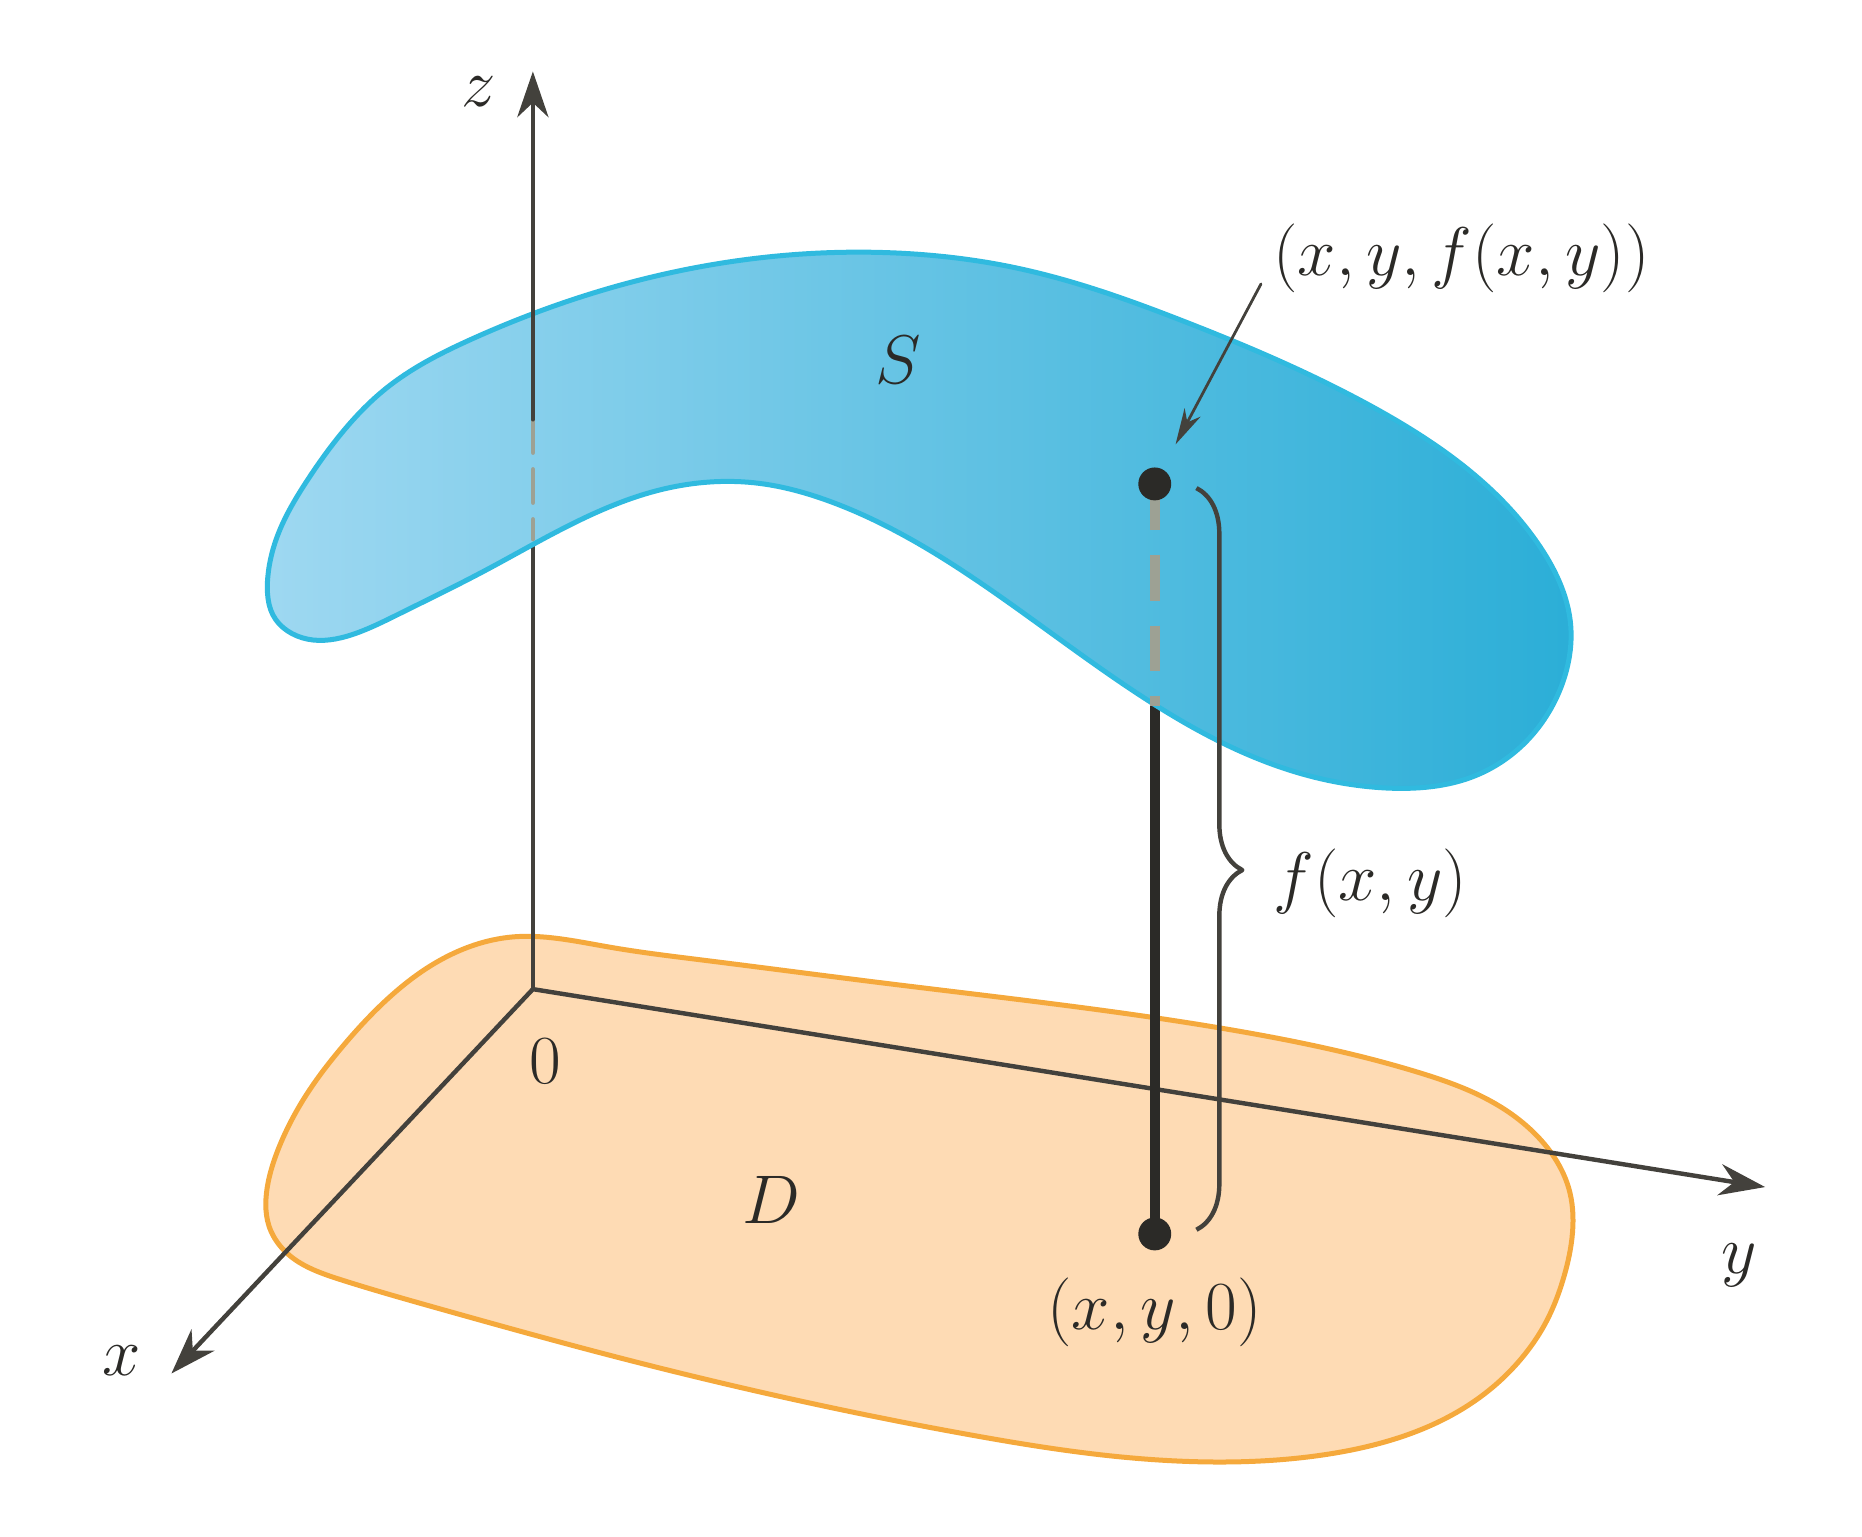
\begin{tikzpicture}[
    x=0.75bp,y=-0.75bp,
    line cap=round,line join=round,
    every node/.style={inner sep=0pt,outer sep=0pt,text=ink,
      font=\fontsize{33bp}{36bp}\selectfont},
    axis/.style={draw=axisink,ultra thick,
      -{Stealth[length=16.5bp,width=11.25bp,inset=5.25bp]}},
    projection/.style={draw=ink,line width=3.75bp,line cap=butt},
    hidden projection/.style={projection,draw=hiddenink,
      dash pattern=on 16.5bp off 9bp},
    height brace/.style={draw=axisink,ultra thick,line cap=butt,
      decorate,decoration={brace,amplitude=16.5bp,aspect=0.515}},
    leader/.style={draw=axisink,line width=1bp,
      -{Stealth[length=13bp,width=6.5bp,inset=4bp]}},
    dot/.style={fill=ink,draw=none}
  ]
  % Preserve the reference canvas and margins.
  \path[use as bounding box] (0,0) rectangle (867,711);
  \clip (0,0) rectangle (867,711);

  \coordinate (Origin) at (242.5,461.5);
  \coordinate (Xtip) at (69,646);
  \coordinate (Ytip) at (834,556.5);
  \coordinate (Ztip) at (242.5,21);
  \coordinate (SurfacePoint) at (541,219);
  \coordinate (BasePoint) at (541,579);
  \coordinate (ProjectionRim) at (541,325.5);
  \coordinate (Zfront) at (242.5,245.5);
  \coordinate (Zhidden) at (242.5,188);
  \coordinate (BraceTop) at (561,221);
  \coordinate (BraceBottom) at (561,577);

  % 1. Domain, planar axes and vertical lines behind the surface.
  \path[fill=domainfill,draw=domainrim,line width=1.8bp] \domainoutline;
  \draw[axis] (Origin) -- (Xtip);
  \draw[axis] (Origin) -- (Ytip);
  \draw[draw=axisink,ultra thick] (Origin) -- (Zfront);
  \draw[projection] (ProjectionRim) -- (BasePoint);

  % 2. Surface: a single gradient controlled by surfaceleft / surfaceright.
  \shadedraw[left color=surfaceleft,right color=surfaceright,
    draw=surfacerim,line width=1.8bp] \surfaceoutline;

  % 3. Visible and hidden vertical segments, and the two marked points.
  \draw[draw=hiddenink,ultra thick,
    dash pattern=on 12bp off 6bp] (Zhidden) -- (Zfront);
  \draw[axis] (Zhidden) -- (Ztip);
  \draw[hidden projection,dash phase=0bp]
    (SurfacePoint) -- (ProjectionRim);
  \path[dot] (SurfacePoint) circle[radius=7.9];
  \path[dot] (BasePoint) circle[radius=7.9];

  % 4. One continuous native brace.
  \draw[height brace] (BraceTop) -- (BraceBottom);

  % 5. Baseline-anchored labels, independent of the geometric paths.
  \draw[leader] (592,123) -- (551,200);
  \node[anchor=base west] at (208,38) {$z$};
  \node[anchor=base west] at (36,647) {$x$};
  \node[anchor=base west] at (813,598) {$y$};
  \node[anchor=base west] at (241,507) {$0$};
  \node[anchor=base west] at (407,171) {$S$};
  \node[anchor=base west] at (343,574) {$D$};
  \node[anchor=base west] at (598,119) {$(x,y,f(x,y))$};
  \node[anchor=base west] at (598,419) {$f(x,y)$};
  \node[anchor=base] at (541,625) {$(x,y,0)$};
\end{tikzpicture}
\end{document}
